\subsubsection{Drehmoment}

\begin{itemize}
	\item Die wirksame Hebellänge wird begrenzt zwischen dem Drehpunkt und dem Ansatzpunkt der Kraft
	\item Mehrere Drehmomente im Gegenuhrzeigersinn (positives Vorzeichen) und im Uhrzeigersinn (Vorzeichen) sind im Gleichgewicht, wenn das Gesamtdrehmoment $M_{tot}$ null ist.
	\item \textbf{Hebelgesetz}: Kraft $\cdot$ Kraftarm = Last $\cdot$ Lastarm
	\item Der Bezugspunkt P ist frei wählbar
	\item Das Drehmoment ($M = J \alpha$) ist für die Rotation, die Kraft in der Translation ($F = ma$)
\end{itemize}

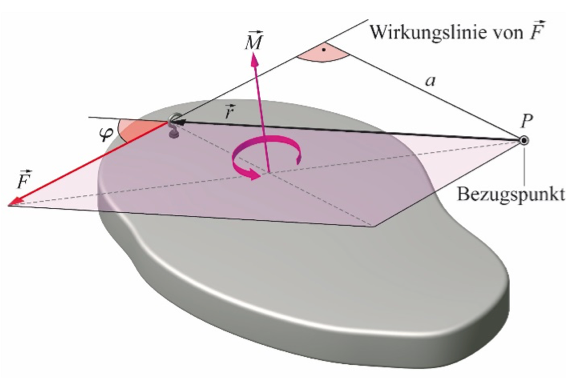
\includegraphics[width=0.4\linewidth]{images/drehmoment}

\begin{tabbing}
	\begin{tabu} to \linewidth {l X l X}
		\toprule
		Hebelgesetz & $F_1l_1 = F_2l_2 \Leftrightarrow M_1 = M_2$ & 
		Drehmoment & $M = F \cdot r \cdot \sin(\varphi)$ \\
		Drehmoment & $M = J \cdot \alpha$ & 
		Trägheitsmoment & $J = m r^2$ \\
	\end{tabu}
\end{tabbing}

\begin{tabbing}
	\begin{tabu} to \linewidth {l X l}
		Variable & Bedeutung & SI-Einheit \\
		\midrule
		$M$ & Drehmoment & $Nm$ \\ 
		$F$ & wirkende Kraft & $Nm$ \\ 
		$r$ & Abstand Bezugspunkt-Angriffspunkt & $m$ \\ 
		$a$ & Hebelarm: senkrechter Abstand Bezugspunkt-Wirkungslinie der Kraft & $m$ \\ 
		$P$ & Bezugspunkt: Frei wählbar & \\
		\bottomrule
	\end{tabu}
\end{tabbing}


\begin{minipage}[h!]{0.5\linewidth}
	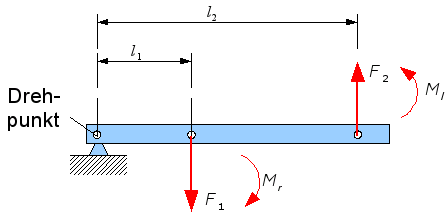
\includegraphics[width=0.8\linewidth]{images/hebel_einseitig}
\end{minipage}
\hfill
\begin{minipage}[h!]{0.5\linewidth}
	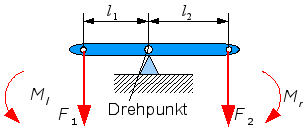
\includegraphics[width=0.8\linewidth]{images/hebel_zweiseitig}
\end{minipage}



\begin{minipage}[h!]{0.5\linewidth}
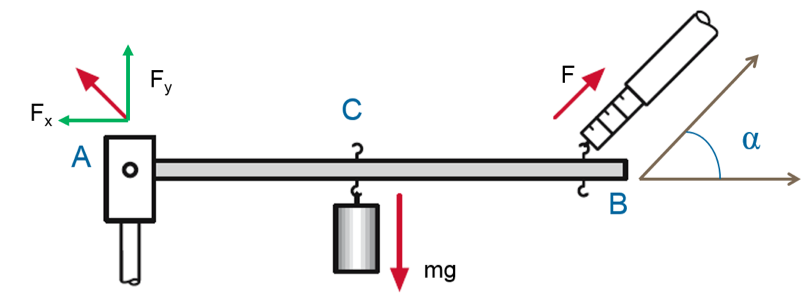
\includegraphics[width=0.9\linewidth]{images/hebel}
\end{minipage}
\hfill
\begin{minipage}[h!]{0.5\linewidth}
	
	\begin{align*}
	M_A &:	F  \cdot r \cdot  \sin(\alpha) - m g \cdot \frac{r}{2} = 0 \\
	\Rightarrow F &= \frac{mg}{2 \sin(\alpha)} \\
	X&:	F \cos(\alpha) - F_x = 0 \\ 
	Y&:	F \sin(\alpha) + F_y - m g = 0 \\ 
	\Rightarrow F_x &= F \cos(\alpha) \text{ und } F_y = mg - F \sin(\alpha) \\
	\Rightarrow F_{t} &= F_1 + F_2 \\
	\end{align*}
	
\end{minipage}